\documentclass[a4paper,12pt]{article}
\usepackage{bbding,combelow,textcomp,amsfonts,amsthm,amsmath,amssymb,graphicx,color,hyperref,etoolbox}
\usepackage[utf8x]{inputenc}
\usepackage[lined,boxed,commentsnumbered]{algorithm2e}
\usepackage{tikz}
\usetikzlibrary{calc,decorations.pathreplacing}

\newtoggle{story}


%%%%%%%%%%%%%%%%%%%%%%%%%%%%%%%%%%%%%%%%%%
%% Customisation options --- update as necessary
%%%%%%%%%%%%%%%%%%%%%%%%%%%%%%%%%%%%%%%%%%

%% Course details: title, semester, instructors

\newcommand{\courseTitle}{Probabilistic Combinatorics (Math 5390)}
\newcommand{\semester}{Fall 2026}
\newcommand{\instructorA}{Shagnik Das}
\newcommand{\instructorB}{}

%% Sheet number

\newcommand{\sheetNumber}{1}


%% Submission details

\newcommand{\dueDate}{15:30, Oct 6th.}
\newcommand{\lateWarning}{Late submissions will receive no credit.}


%% Display irrelevant footnotes?  \toggletrue for yes, \togglefalse for no

\toggletrue{story}

%%%%%%%%%%%%%%%%%%%%%%%%%%%%%%%%%%%%%%%%%%
%% End of customisation options
%%%%%%%%%%%%%%%%%%%%%%%%%%%%%%%%%%%%%%%%%%

\pdfpagewidth 8.5in
\pdfpageheight 11in
\topmargin -1in
\headheight 0in
\headsep 0in
\textheight 8.5in
\textwidth 6.5in
\oddsidemargin 0in
\evensidemargin 0in
\headheight 77pt
\headsep 0in
\footskip .75in

\makeatletter
\newcommand{\buildtitle}[4]{
\begin{flushleft}
{\large
#1
\hfill{}
#2
\par
#3
}
\end{flushleft}
\vskip 4pt
\begin{center}
{\large\bfseries#4\par}
\end{center}
\bigskip
}
\makeatother

\renewcommand{\thesection}{\normalsize\arabic{section}}

\renewcommand{\deg}{\textrm{deg}}
\newcommand{\eps}{\varepsilon}
\newcommand{\ceil}[1]{\left \lceil #1 \right \rceil}

\newcommand{\hint}{\begin{flushright} [Hint at \url{\hintURL}.] \end{flushright}}

\newcommand{\card}[1]{\left| #1 \right|}
\newcommand{\mb}[1]{\mathbb{#1}}
\newcommand{\mc}[1]{\mathcal{#1}}


\newcommand{\story}[1]{\iftoggle{story}{\footnote{#1}}{}}
\newcommand{\storymark}[1][42]{\iftoggle{story}{\footnotemark[#1]}{}}
\newcommand{\storytext}[2][42]{\iftoggle{story}{\footnotetext[#1]{#2}}{}}

\newcommand{\bonus}[2]{\paragraph{Bonus (#1 pt\ifstrequal{#1}{1}{}{s})} #2}


\begin{document}


\buildtitle{\courseTitle{}}{\semester}{\instructorA{} \hfill \instructorB{}}{Exercise Sheet \sheetNumber{}}

\vspace{-0.2in}

\begin{center}

{\bf Due date: \dueDate \\ \lateWarning}

\end{center}

\noindent You and your partner should try to solve all of the exercises below, and then submit a total of two solutions to be graded --- each problem is worth $10$ points. Both partners should author one solution each, making clear who wrote which solution, but you will earn credit for both solutions. Make sure to clearly justify your answers, defining everything precisely and stating any results you are using. You should then submit your solutions on NTU COOL, either as a typed PDF or a clear picture or scan of your handwritten answers.

\paragraph{Exercise 1}  Given natural numbers $k, \ell$, we define the asymmetric Ramsey number $R(k,\ell)$ as the smallest $n$ such that every red-/blue-colouring of the edges of $K_n$ contains a red $K_k$ or a blue $K_{\ell}$.
\begin{itemize}
	\item[(a)] Show that for $k, \ell \ge 2$, we have $R(k, \ell) \le R(k, \ell-1) + R(k-1, \ell)$.
	\item[(b)] Deduce that for $k, \ell \ge 1$, we have $R(k, \ell) \le \binom{k + \ell - 2}{k-1}$.
	\item[(c)] Sharpen this bound to show $R(3,4) \le 9$.
\end{itemize}

\paragraph{Solution (to be graded; authored by Chang).} Throughout, note that $R(1, \ell) = R(k, 1) = 1$, since $K_1$ has no edges and hence is trivially both a red $K_1$ and a blue $K_1$.

\begin{proof}[Proof of (a)]
	If $R(k, \ell - 1)$ or $R(k-1, \ell)$ is infinite there is nothing to prove, so assume both are finite and let $n = R(k, \ell-1) + R(k-1, \ell)$. Take an arbitrary red-/blue-colouring of the edges of $K_n$ and fix a vertex $v$. Let $N_R$ (resp.\ $N_B$) be the set of vertices joined to $v$ by a red (resp.\ blue) edge. Then $\card{N_R} + \card{N_B} = n - 1$, so either $\card{N_R} \ge R(k-1, \ell)$ or $\card{N_B} \ge R(k, \ell-1)$; otherwise $n - 1 \le R(k-1,\ell) + R(k,\ell-1) - 2 = n - 2$, a contradiction.

	\begin{center}
	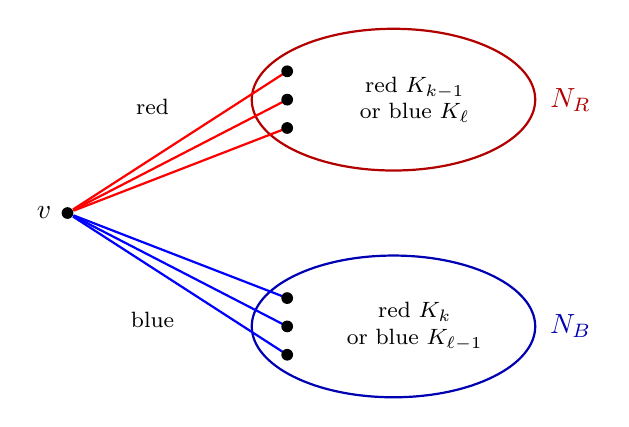
\begin{tikzpicture}[vtx/.style={circle,fill=black,inner sep=1.5pt}, scale=0.9]
		\node[vtx,label=left:$v$] (v) at (0,0) {};
		\draw[thick,red!70!black] (4.6,1.6) ellipse (2 and 1);
		\draw[thick,blue!70!black] (4.6,-1.6) ellipse (2 and 1);
		\node[red!70!black] at (7.1,1.6) {$N_R$};
		\node[blue!70!black] at (7.1,-1.6) {$N_B$};
		\foreach \y in {1.2,1.6,2.0} {\draw[red,thick] (v) -- (3.1,\y); \node[vtx] at (3.1,\y) {};}
		\foreach \y in {-1.2,-1.6,-2.0} {\draw[blue,thick] (v) -- (3.1,\y); \node[vtx] at (3.1,\y) {};}
		\node[font=\footnotesize,align=center] at (4.9,1.6) {red $K_{k-1}$\\or blue $K_\ell$};
		\node[font=\footnotesize,align=center] at (4.9,-1.6) {red $K_{k}$\\or blue $K_{\ell-1}$};
		\node[font=\footnotesize] at (1.2,1.5) {red};
		\node[font=\footnotesize] at (1.2,-1.5) {blue};
	\end{tikzpicture}
	\end{center}

	\emph{Case 1: $\card{N_R} \ge R(k-1, \ell)$.} The colouring restricted to the complete graph on $N_R$ contains a red $K_{k-1}$ or a blue $K_\ell$. A blue $K_\ell$ is what we want. If it contains a red $K_{k-1}$, then adding $v$, which is joined to all of its vertices by red edges, gives a red $K_k$.

	\emph{Case 2: $\card{N_B} \ge R(k, \ell-1)$.} Symmetrically, the complete graph on $N_B$ contains a red $K_k$, or a blue $K_{\ell-1}$, which together with $v$ forms a blue $K_\ell$.

	Hence every colouring of $K_n$ contains a red $K_k$ or a blue $K_\ell$, so $R(k,\ell) \le n = R(k, \ell-1) + R(k-1, \ell)$.
\end{proof}

\begin{proof}[Proof of (b)]
	We induct on $k + \ell$. If $k = 1$ or $\ell = 1$, then $R(k, \ell) = 1 = \binom{k+\ell-2}{k-1}$, since $\binom{\ell-1}{0} = \binom{k-1}{k-1} = 1$. Now let $k, \ell \ge 2$ and assume the claim for all pairs with smaller sum. In particular $R(k,\ell-1)$ and $R(k-1,\ell)$ are finite, and by (a) and Pascal's rule,
	\[
		R(k, \ell) \le R(k, \ell - 1) + R(k-1, \ell) \le \binom{k + \ell - 3}{k-1} + \binom{k + \ell - 3}{k - 2} = \binom{k + \ell - 2}{k-1}.
	\]
\end{proof}

\begin{proof}[Proof of (c)]
	By (b), $R(3,3) \le \binom{4}{2} = 6$. Suppose, for contradiction, that some colouring of $K_9$ has neither a red $K_3$ nor a blue $K_4$. Fix a vertex $v$ and define $N_R, N_B$ as in (a), so $\card{N_R} + \card{N_B} = 8$.

	\begin{center}
	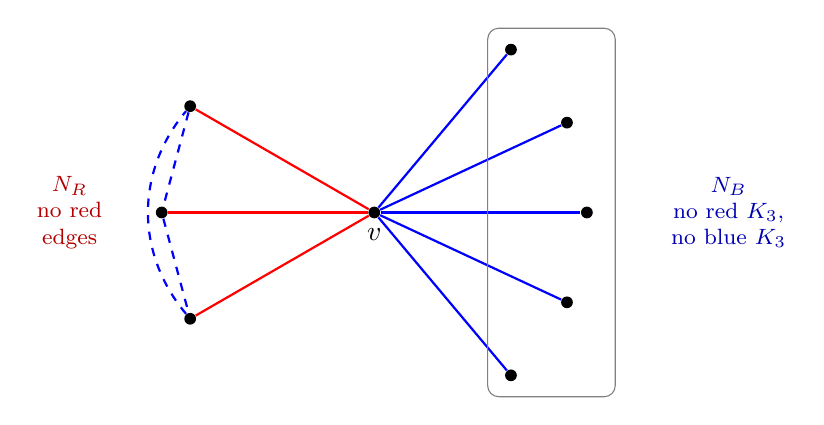
\begin{tikzpicture}[vtx/.style={circle,fill=black,inner sep=1.5pt}, scale=0.9]
		\node[vtx,label=below:$v$] (v) at (0,0) {};
		% red neighbourhood: 3 vertices, all edges among them blue
		\foreach \i/\a in {1/150,2/180,3/210} \node[vtx] (r\i) at ($(v)+(\a:3)$) {};
		\foreach \i in {1,2,3} \draw[red,thick] (v) -- (r\i);
		\draw[blue,thick,dashed] (r1) -- (r2) -- (r3) to[bend left=40] (r1);
		\node[red!70!black,align=center,font=\footnotesize] at (-4.3,0) {$N_R$\\no red\\edges};
		% blue neighbourhood: 5 vertices
		\foreach \i/\a in {1/50,2/25,3/0,4/-25,5/-50} \node[vtx] (b\i) at ($(v)+(\a:3)$) {};
		\foreach \i in {1,...,5} \draw[blue,thick] (v) -- (b\i);
		\draw[gray,rounded corners] (1.6,-2.6) rectangle (3.4,2.6);
		\node[blue!70!black,align=center,font=\footnotesize] at (5,0) {$N_B$\\no red $K_3$,\\no blue $K_3$};
	\end{tikzpicture}
	\end{center}

	\begin{itemize}
		\item $\card{N_R} \le 3$: if $x, y \in N_R$ were joined by a red edge, then $\{v, x, y\}$ would be a red $K_3$. So all edges inside $N_R$ are blue, and if $\card{N_R} \ge 4$, any four vertices of $N_R$ form a blue $K_4$.
		\item $\card{N_B} \le 5$: if $\card{N_B} \ge 6 \ge R(3,3)$, then $N_B$ contains a red $K_3$, or a blue $K_3$, which together with $v$ forms a blue $K_4$.
	\end{itemize}
	Thus $\card{N_R} = 8 - \card{N_B} \ge 3$, so $\card{N_R} = 3$. That is, every vertex is incident to exactly $3$ red edges, so the red edges form a $3$-regular graph on $9$ vertices. But by the handshake lemma the sum of degrees, $9 \cdot 3 = 27$, must equal twice the number of red edges, which is impossible since $27$ is odd. Hence every colouring of $K_9$ contains a red $K_3$ or a blue $K_4$, i.e.\ $R(3,4) \le 9$.
\end{proof}

\paragraph{Exercise 2}  Let $H$ be a $k$-uniform hypergraph on $n$ vertices $V$ with edges $E = \{ e_1, e_2, \hdots, e_m \}$. To each vertex $v \in V$, associate a uniformly random number $x(v) \in [0,1]$. Order the vertices in increasing order of the numbers $x(v)$, and colour them greedily --- colour the vertex red, unless it would create an all-red edge, in which case colour it blue.

Fix some $\varepsilon > 0$, and consider the following events:
\begin{itemize}
	\item $E_i$: the event that for every vertex $v$ in the edge $e_i$, we have $x(v) \le \frac12(1- \varepsilon)$.
	\item $L_i$: the event that for every vertex $v$ in the edge $e_i$, we have $x(v) \ge \frac12(1 + \varepsilon)$.
	\item $M_{i,j}$: the event that edges $e_i$ and $e_j$ have a single common vertex $w$, with $\frac12(1 - \varepsilon) < x(w) < \frac12(1 + \varepsilon)$, and that for every vertex $u \in e_i$ we have $x(u) \le x(w)$, and for every vertex $v \in e_j$ we have $x(v) \ge x(w)$.
\end{itemize}

\begin{itemize}
	\item[(a)] Show that $H$ has Property B (i.e. is two-colourable), unless the event $\left( \cup_{i \in [m]} E_i \right) \cup \left( \cup_{i \in [m]} L_i \right) \cup \left( \cup_{i,j \in [m]} M_{i,j} \right)$ occurs.
	\item[(b)] Bound the probability of this event in terms of $m$ and $\varepsilon$.
	\item[(c)] By choosing $\varepsilon$ appropriately, show that $m(k) \ge c \left( \frac{k}{\log k} \right)^{1/2} 2^k$, for some constant $c > 0$.
\end{itemize}

\paragraph{Solution.} Throughout we assume $k \ge 2$. Recall that $H$ has Property B if its vertices can be coloured red and blue with no monochromatic edge, and $m(k)$ denotes the minimum number of edges in a $k$-uniform hypergraph without Property B. We write $\mathcal{B} = \left( \cup_{i} E_i \right) \cup \left( \cup_{i} L_i \right) \cup \left( \cup_{i,j} M_{i,j} \right)$ for the bad event.

\begin{proof}[Proof of (a)]
	Process the vertices in increasing order of $x(v)$ (breaking ties arbitrarily), and colour them greedily as described. We say $u$ comes \emph{before} $w$ if $u$ is processed before $w$; in that case $x(u) \le x(w)$.

	\emph{No edge is all red.} Suppose $e$ were all red, and let $v$ be the last vertex of $e$ to be processed. When $v$ was coloured, all other vertices of $e$ were already red, so colouring $v$ red would create an all-red edge, and the rule would have coloured $v$ blue. Contradiction.

	\emph{If some edge is all blue, then $\mathcal{B}$ occurs.} Suppose $e_j$ is all blue, and let $w$ be the first vertex of $e_j$ to be processed. Since $w$ is blue, colouring it red would have created an all-red edge: there is an edge $e_i \ni w$ such that every vertex of $e_i \setminus \{w\}$ was processed before $w$ and coloured red. We claim:
	\begin{itemize}
		\item $e_i \cap e_j = \{w\}$. Indeed, if $u \ne w$ lies in both, then $u$ comes before $w$ (as $u \in e_i \setminus \{w\}$) and after $w$ (as $w$ is the first vertex of $e_j$), which is impossible. In particular $e_i \ne e_j$, as $k \ge 2$.
		\item $x(u) \le x(w)$ for all $u \in e_i$, since all of $e_i$ is processed no later than $w$; and $x(v) \ge x(w)$ for all $v \in e_j$, since $w$ is the first vertex of $e_j$.
	\end{itemize}
	Now we distinguish three cases according to the position of $x(w)$; see Figure~\ref{fig:ex2}.
	\begin{itemize}
		\item If $x(w) \le \frac12(1-\eps)$, then every $u \in e_i$ has $x(u) \le x(w) \le \frac12(1-\eps)$, so $E_i$ occurs.
		\item If $x(w) \ge \frac12(1+\eps)$, then every $v \in e_j$ has $x(v) \ge x(w) \ge \frac12(1+\eps)$, so $L_j$ occurs.
		\item Otherwise $\frac12(1-\eps) < x(w) < \frac12(1+\eps)$, and together with the two bullet points above, this is exactly the event $M_{i,j}$.
	\end{itemize}
	Hence if $\mathcal{B}$ does not occur, the greedy colouring has neither an all-red nor an all-blue edge, so $H$ has Property B.
\end{proof}

\begin{figure}[ht]
\centering
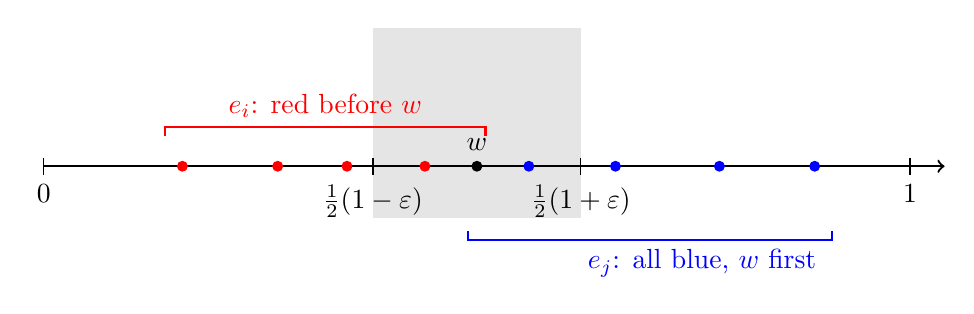
\begin{tikzpicture}[scale=1.1, vtx/.style={circle,fill=black,inner sep=1.4pt}]
	\fill[gray!20] (3.8,-0.6) rectangle (6.2,1.6);
	\draw[thick,->] (0,0) -- (10.4,0);
	\foreach \x/\l in {0/$0$, 10/$1$} {\draw (\x,0.1) -- (\x,-0.1); \node[below] at (\x,-0.1) {\l};}
	\draw (3.8,0.1) -- (3.8,-0.1); \node[below] at (3.8,-0.1) {$\frac12(1-\eps)$};
	\draw (6.2,0.1) -- (6.2,-0.1); \node[below] at (6.2,-0.1) {$\frac12(1+\eps)$};
	% the common vertex w
	\node[vtx,label=above:$w$] (w) at (5,0) {};
	% e_i to the left (red), e_j to the right (blue)
	\foreach \x in {1.6,2.7,3.5,4.4} \node[vtx,red] at (\x,0) {};
	\foreach \x in {5.6,6.6,7.8,8.9} \node[vtx,blue] at (\x,0) {};
	\draw[red,thick] (1.4,0.35) -- (1.4,0.45) -- (5.1,0.45) -- (5.1,0.35);
	\node[red,above] at (3.25,0.45) {$e_i$: red before $w$};
	\draw[blue,thick] (4.9,-0.75) -- (4.9,-0.85) -- (9.1,-0.85) -- (9.1,-0.75);
	\node[blue,below] at (7.6,-0.85) {$e_j$: all blue, $w$ first};
\end{tikzpicture}
\caption{The configuration in (a). The shaded strip is the middle range of $x(w)$, giving $M_{i,j}$; if $x(w)$ lies left of it then $E_i$ occurs, and if right of it then $L_j$ occurs.}
\label{fig:ex2}
\end{figure}

\begin{proof}[Proof of (b)]
	Each $x(v)$ lies below $\frac12(1-\eps)$, or above $\frac12(1+\eps)$, with probability $\frac{1-\eps}{2}$, so by independence
	\[
		\Pr(E_i) = \Pr(L_i) = \left( \tfrac{1-\eps}{2} \right)^k.
	\]
	For $M_{i,j}$, note that $H$ is fixed, so $|e_i \cap e_j|$ is not random, and we split into two cases.

	\emph{Case 1: $|e_i \cap e_j| \ne 1$.} By definition, $M_{i,j}$ requires $e_i$ and $e_j$ to have exactly one common vertex, so $M_{i,j} = \emptyset$ and $\Pr(M_{i,j}) = 0$. This includes $i = j$, as $k \ge 2$. (Even if one only asks for \emph{some} common vertex $w$ satisfying the conditions, any other common vertex $u$ would satisfy $x(w) \le x(u) \le x(w)$, i.e.\ $x(u) = x(w)$, which has probability $0$.)

	\emph{Case 2: $e_i \cap e_j = \{w\}$.} Let $I = \left( \frac12(1-\eps), \frac12(1+\eps) \right)$. By the law of total probability, conditioning on $x(w)$,
	\[
		\Pr(M_{i,j}) = \int_0^1 \Pr\left( M_{i,j} \mid x(w) = t \right) dt.
	\]
	Given $x(w) = t$, the event $M_{i,j}$ occurs if and only if $t \in I$, all $k-1$ values $x(u)$, $u \in e_i \setminus \{w\}$, are at most $t$, and all $k-1$ values $x(v)$, $v \in e_j \setminus \{w\}$, are at least $t$. The sets $e_i \setminus \{w\}$ and $e_j \setminus \{w\}$ are disjoint and do not contain $w$, so these $2(k-1)$ values are independent of each other and of $x(w)$. Hence
	\[
		\Pr\left( M_{i,j} \mid x(w) = t \right) = \mathbf{1}[t \in I] \, t^{k-1} (1-t)^{k-1},
	\]
	and therefore
	\[
		\Pr(M_{i,j}) = \int_I t^{k-1} (1-t)^{k-1} \, dt \le \eps \cdot \left( \tfrac14 \right)^{k-1},
	\]
	because $I$ has length $\eps$ and $t(1-t) \le \frac14$ for all $t$.

	In both cases $\Pr(M_{i,j}) \le \eps \, 4^{1-k}$. Finally, $\mathcal{B}$ is the union of the $m$ events $E_i$, the $m$ events $L_i$ and the $m^2$ events $M_{i,j}$ ($i, j \in [m]$), so by the union bound
	\[
		\Pr(\mathcal{B}) \le \sum_{i=1}^m \Pr(E_i) + \sum_{i=1}^m \Pr(L_i) + \sum_{i,j=1}^m \Pr(M_{i,j}) \le m \left( \tfrac{1-\eps}{2} \right)^k + m \left( \tfrac{1-\eps}{2} \right)^k + m^2 \cdot \eps \, 4^{1-k},
	\]
	that is,
	\[
		\Pr(\mathcal{B}) \le 2m \left( \tfrac{1-\eps}{2} \right)^k + m^2 \eps \, 4^{1-k}.
	\]
\end{proof}

\begin{proof}[Proof of (c)]
	Logarithms here are natural; since $\log_2 k > \ln k$, the bound with $\ln$ implies the one with $\log_2$. Let $c = \frac14$, fix $k \ge 3$, and suppose $H$ has $m \le c\, 2^k (k / \ln k)^{1/2}$ edges. Take $\eps = \frac{\ln k}{2k} \in (0,1)$. Using $1 - \eps \le e^{-\eps}$, we get $(1-\eps)^k \le e^{-\eps k} = k^{-1/2}$, so by (b),
	\begin{align*}
		\Pr(\mathcal{B}) &\le 2 m 2^{-k} k^{-1/2} + 4 \eps m^2 4^{-k} \\
		&\le 2c \left( \frac{k}{\ln k} \right)^{1/2} k^{-1/2} + 4 \cdot \frac{\ln k}{2k} \cdot c^2 \frac{k}{\ln k} = \frac{2c}{\sqrt{\ln k}} + 2c^2 \le \frac12 + \frac18 < 1,
	\end{align*}
	using $\ln k \ge \ln 3 > 1$. Hence with positive probability $\mathcal{B}$ fails, and by (a) $H$ has Property B. Therefore every $k$-uniform hypergraph without Property B has more than $c\, 2^k (k/\ln k)^{1/2}$ edges, i.e.
	\[
		m(k) > \tfrac14 \left( \frac{k}{\ln k} \right)^{1/2} 2^k \qquad \text{for all } k \ge 3.
	\]
	This also holds for $k = 2$: a graph without Property B is non-bipartite, so it has an odd cycle and $m(2) = 3 > \frac14 \cdot (2/\ln 2)^{1/2} \cdot 4 \approx 1.70$.
\end{proof}

\paragraph{Exercise 3}  Show that there is some constant $c > 0$ such that, if $n$ is sufficiently large and every vertex of an $n$-vertex graph $G$ has degree at least $\log n - c \log \log n$, then we can colour the vertices of $G$ red and blue in such a way that every vertex has both a red neighbour and a blue neighbour.

\paragraph{Solution.} Throughout, $\log$ denotes $\log_2$ and $\ln$ the natural logarithm, and we show that $c = \frac14$ works. As in Exercise 2, $m(k)$ denotes the minimum number of edges in a $k$-uniform hypergraph without Property B. We also write
\[
	g(x) = 2^x \left( \frac{x}{\ln x} \right)^{1/2}.
\]
By Exercise 2(c), $m(k) > \frac14 g(k)$ for every $k \ge 2$. Equivalently,
\begin{equation}\label{eq:mk}
	\text{every $k$-uniform hypergraph with at most $\tfrac14 g(k)$ edges has Property B} \qquad (k \ge 2).
\end{equation}

\begin{proof}
	Let $G$ be a graph on $n$ vertices whose minimum degree $\delta$ satisfies
	\[
		\delta \ge L := \log n - \tfrac14 \log\log n.
	\]

	\emph{Step 1: the hypergraph $H$.} For each vertex $v$, choose a set $S_v \subseteq N(v)$ of exactly $\delta$ neighbours of $v$. This is possible since $\deg(v) \ge \delta$. Let $H$ be the hypergraph on $V(G)$ with edge set $\{ S_v : v \in V(G) \}$. Then $H$ is $\delta$-uniform and has at most $n$ edges (one for each vertex, possibly with repetitions).

	\emph{Step 2: if $H$ has Property B, we are done.} Suppose $H$ has Property B, so there is a red/blue colouring of $V(G)$ in which no edge $S_v$ of $H$ is monochromatic. Then for every vertex $v$, the set $S_v$ contains a red vertex and a blue vertex. Since $S_v \subseteq N(v)$, these are a red neighbour and a blue neighbour of $v$ (see Figure~\ref{fig:ex3}).

	\emph{Step 3: $H$ has Property B for all large $n$.} By \eqref{eq:mk} applied with $k = \delta$, and since $H$ has at most $n$ edges, it suffices to show that $\delta \ge 2$ and
	\[
		n \le \tfrac14\, g(\delta).
	\]
	\begin{itemize}
		\item[(a)] \emph{$g$ is increasing on $[e, \infty)$.} We have $\frac{d}{dx} \frac{x}{\ln x} = \frac{\ln x - 1}{(\ln x)^2} \ge 0$ for $x \ge e$. So $x / \ln x$ is increasing there, and so is $g(x) = 2^x (x/\ln x)^{1/2}$, as a product of positive increasing functions.
		\item[(b)] \emph{Replace $\delta$ by $L$.} For large $n$ we have $\frac14 \log\log n \le \frac12 \log n$, so
		\[
			\delta \ge L \ge \tfrac12 \log n \ge e.
		\]
		In particular $\delta \ge 2$, and by (a), $g(\delta) \ge g(L)$.
		\item[(c)] \emph{Compute $g(L)$.} On the one hand, $2^L = 2^{\log n} \cdot 2^{-\frac14 \log\log n} = n (\log n)^{-1/4}$. On the other hand, since $L \ge \frac12 \log n \ge e$ and $x / \ln x$ is increasing,
		\[
			\frac{L}{\ln L} \ge \frac{\frac12 \log n}{\ln\left( \frac12 \log n \right)} \ge \frac{\frac12 \log n}{\ln \log n}.
		\]
		Therefore
		\[
			\tfrac14\, g(L) = \tfrac14 \cdot 2^L \cdot \left( \frac{L}{\ln L} \right)^{1/2} \ge \tfrac14 \cdot n (\log n)^{-1/4} \cdot \frac{(\log n)^{1/2}}{(2 \ln \log n)^{1/2}} = n \cdot \frac{(\log n)^{1/4}}{4 \sqrt{2 \ln \log n}}.
		\]
		The last fraction tends to infinity as $n \to \infty$, since a positive power of $\log n$ grows faster than $\sqrt{\ln \log n}$. So it is at least $1$ for all large $n$, and then $\frac14 g(L) \ge n$.
	\end{itemize}
	Combining (b) and (c), $\frac14 g(\delta) \ge \frac14 g(L) \ge n$ for all large $n$. So $H$ has Property B by Step 3, and $G$ has the required colouring by Step 2.
\end{proof}

\begin{figure}[ht]
\centering
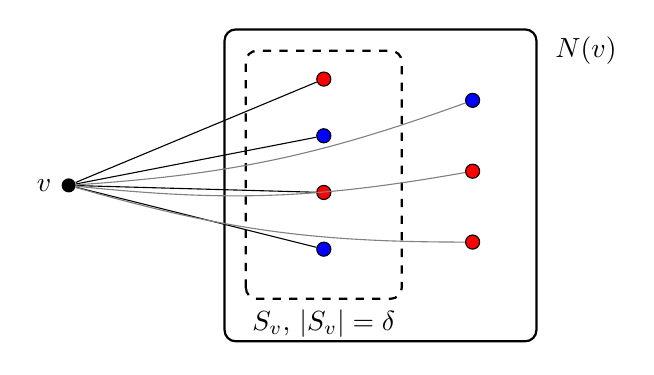
\begin{tikzpicture}[vtx/.style={circle,draw,inner sep=1.8pt}, scale=0.9]
	\node[circle,fill=black,inner sep=1.8pt,label=left:$v$] (v) at (0,0) {};
	\draw[thick,rounded corners] (2.2,-2.2) rectangle (6.6,2.2);
	\node at (7.3,1.9) {$N(v)$};
	\draw[thick,dashed,rounded corners] (2.5,-1.6) rectangle (4.7,1.9);
	\node at (3.6,-1.95) {$S_v$, $|S_v| = \delta$};
	\foreach \y/\c [count=\i] in {1.5/red, 0.7/blue, -0.1/red, -0.9/blue} {
		\node[vtx,fill=\c] (a\i) at (3.6,\y) {};
		\draw (v) -- (a\i);
	}
	\foreach \y/\c [count=\i] in {1.2/blue, 0.2/red, -0.8/red} {
		\node[vtx,fill=\c] (b\i) at (5.7,\y) {};
		\draw[gray] (v) to[bend right=8] (b\i);
	}
\end{tikzpicture}
\caption{Each $S_v \subseteq N(v)$ is an edge of $H$. If no edge of $H$ is monochromatic, then $v$ sees both colours in $N(v)$.}
\label{fig:ex3}
\end{figure}

\paragraph{Exercise 4}  Prove that there is some constant $c > 0$ such that if a tournament has the $k$-Sch\"utte property, it must have at least $c k 2^k$ vertices.

\paragraph{Solution.} We write $u \to w$ if $u$ beats $w$. A tournament $T$ has the $k$-Sch\"utte property if it has more than $k$ vertices and for every set $U$ of $k$ vertices there is a vertex $z \notin U$ with $z \to u$ for all $u \in U$. For a set $U$, let
\[
	D(U) = \{ z \notin U : z \to u \text{ for all } u \in U \}
\]
be the set of \emph{dominators} of $U$ (so $D(\emptyset) = V(T)$). If $|U| \le k$, then $D(U) \ne \emptyset$: extend $U$ to a $k$-set $U' \supseteq U$; any dominator of $U'$ is outside $U$ and beats all of $U$. We prove that $c = \frac12$ works; in fact $n \ge (k+2) 2^{k-1} - 1$.

\begin{proof}
	Let $T$ have the $k$-Sch\"utte property and $n$ vertices.

	\emph{Step 1: every set $S$ of $k-1$ vertices has $|D(S)| \ge k+1$.} Let $Y = D(S)$.
	\begin{itemize}
		\item[(i)] \emph{Every vertex $u \notin S$ is beaten by some $y \in Y$.} The set $S \cup \{u\}$ has $k$ vertices, so it has a dominator $z \notin S \cup \{u\}$. As $z$ beats all of $S$, we have $z \in Y$, and $z \to u$.
		\item[(ii)] \emph{$Y$ has no dominator.} Note $Y \ne \emptyset$ by (i). Suppose $z \notin Y$ beats every vertex of $Y$. If $z \in S$, this is impossible, because every $y \in Y$ beats every vertex of $S$, in particular $y \to z$. If $z \notin S$, then by (i) some $y \in Y$ beats $z$, again a contradiction.
	\end{itemize}
	Since every set of at most $k$ vertices has a dominator, (ii) forces $|Y| \ge k+1$. See Figure~\ref{fig:ex4}.

	\emph{Step 2: a set $S$ of $k-1$ vertices with few dominators.} We choose $v_1, \dots, v_{k-1}$ greedily. Set $D_0 = V(T)$, and for $0 \le i \le k-2$, given $D_i = D(\{v_1, \dots, v_i\})$ (which is non-empty, as $i < k$), note that in the subtournament $T[D_i]$ the in-degrees sum to $\binom{|D_i|}{2}$, so some vertex $v_{i+1} \in D_i$ has in-degree at most $\frac{|D_i| - 1}{2}$ within $D_i$. Since every vertex of $D_i$ already beats $v_1, \dots, v_i$,
	\[
		D_{i+1} := D(\{v_1, \dots, v_{i+1}\}) = \{ y \in D_i : y \to v_{i+1} \},
	\]
	which is exactly the in-neighbourhood of $v_{i+1}$ inside $D_i$. Hence $|D_{i+1}| \le \frac{|D_i| - 1}{2}$, i.e.\ $|D_{i+1}| + 1 \le \frac{|D_i| + 1}{2}$, and by induction
	\[
		|D_{k-1}| + 1 \le \frac{n+1}{2^{k-1}}.
	\]

	\emph{Conclusion.} Applying Step 1 to $S = \{v_1, \dots, v_{k-1}\}$ gives $|D_{k-1}| \ge k+1$, so $k + 2 \le \frac{n+1}{2^{k-1}}$, that is,
	\[
		n \ge (k+2) 2^{k-1} - 1 \ge k\, 2^{k-1} = \tfrac12 k 2^k.
	\]
\end{proof}

\begin{figure}[ht]
\centering
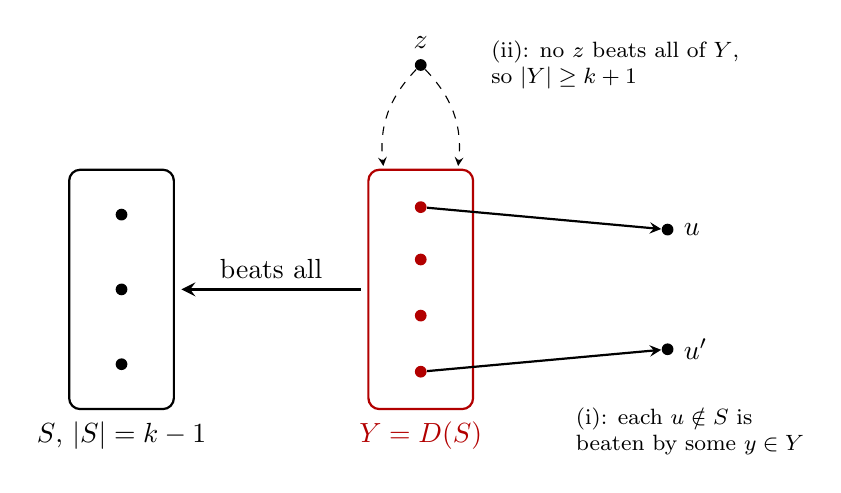
\begin{tikzpicture}[vtx/.style={circle,fill=black,inner sep=1.5pt}, >=stealth, scale=0.95]
	% S
	\draw[thick,rounded corners] (-0.7,-1.6) rectangle (0.7,1.6);
	\node at (0,-1.95) {$S$, $|S| = k-1$};
	\foreach \y in {-1,0,1} \node[vtx] at (0,\y) {};
	% Y
	\draw[thick,rounded corners,red!70!black] (3.3,-1.6) rectangle (4.7,1.6);
	\node[red!70!black] at (4,-1.95) {$Y = D(S)$};
	\foreach \y [count=\i] in {-1.1,-0.35,0.4,1.1} \node[vtx,red!70!black] (y\i) at (4,\y) {};
	\draw[->,very thick] (3.2,0) -- node[above] {beats all} (0.8,0);
	% outside vertices
	\node[vtx,label=right:$u$] (u1) at (7.3,0.8) {};
	\node[vtx,label=right:$u'$] (u2) at (7.3,-0.8) {};
	\draw[->,thick] (y4) -- (u1);
	\draw[->,thick] (y1) -- (u2);
	\node[align=left,font=\footnotesize] at (7.6,-1.9) {(i): each $u \notin S$ is\\beaten by some $y \in Y$};
	% hypothetical dominator of Y
	\node[vtx,label=above:$z$] (z) at (4,3.0) {};
	\draw[->,dashed] (z) to[bend right=25] (3.5,1.65);
	\draw[->,dashed] (z) to[bend left=25] (4.5,1.65);
	\node[font=\footnotesize,align=left] at (6.6,3.0) {(ii): no $z$ beats all of $Y$,\\so $|Y| \ge k+1$};
\end{tikzpicture}
\caption{The two facts in Step 1 for a $(k-1)$-set $S$ and its dominators $Y$.}
\label{fig:ex4}
\end{figure}

\paragraph{Exercise 5}  We say a $k$-uniform hypergraph is rainbow-$r$-colourable if its vertices can be $r$-coloured such that every edge sees all $r$ colours.
\begin{itemize}
	\item[(a)] Prove that if a $k$-uniform hypergraph $H$ has at most $\frac{r^{k-1}}{(r-1)^k}$ edges, then it is rainbow-$r$-colourable.
	\item[(b)] By considering a random hypergraph, or otherwise, show that there exists, for some constant $C = C(r) > 0$ and arbitrarily large $k$, a $k$-uniform hypergraph $H$ with $C k^2 \left( \frac{r}{r-1} \right)^k$ edges that is not rainbow-$r$-colourable.
\end{itemize}

\paragraph{Solution (to be graded; authored by Huang).} Let $r \ge 2$. In a uniformly random $r$-colouring, every vertex independently receives each colour in $[r]$ with probability $\frac1r$. For an edge $e$ and a colour $c$, let $A_{e,c}$ be the event that no vertex of $e$ has colour $c$. An edge is rainbow if and only if none of $A_{e,1}, \dots, A_{e,r}$ occurs.

\begin{proof}[Proof of (a)]
	We may assume $k \ge r$. Indeed, if $k < r$, then an edge of size $k$ cannot see all $r$ colours, so only a hypergraph with no edges is rainbow-$r$-colourable. In this case the statement holds trivially for $r \ge 3$, because then
	\[
		\frac{r^{k-1}}{(r-1)^k} = \frac1r \left( 1 + \frac{1}{r-1} \right)^k \le \frac1r \left( 1 + \frac{1}{r-1} \right)^{r-1} < \frac{e}{r} < 1,
	\]
	so the hypothesis forces $m = 0$. The only remaining case $k < r$ is $r = 2$, $k = 1$, where the bound equals $1$ and the statement fails: a single edge of size $1$ cannot see two colours. From now on let $k \ge r \ge 2$. Let $H$ have $m \le \frac{r^{k-1}}{(r-1)^k}$ edges, and colour $V(H)$ uniformly at random with $r$ colours. If $m = 0$ there is nothing to prove, so let $m \ge 1$. For each edge $e$ and colour $c$,
	since the colours of the $k$ vertices of $e$ are independent,
	\[
		\Pr(A_{e,c}) = \Pr\Big( \bigcap_{v \in e} \{ \text{$v$ is not coloured $c$} \} \Big) = \prod_{v \in e} \Pr(\text{$v$ is not coloured $c$}) = \left( \frac{r-1}{r} \right)^k.
	\]
	The colouring fails to be rainbow exactly when some edge misses some colour, i.e.\ when $\bigcup_{e \in E(H)} \bigcup_{c=1}^{r} A_{e,c}$ occurs. By the union bound over these $mr$ events,
	\begin{align*}
		\Pr(\text{some edge is not rainbow}) &= \Pr\Big( \bigcup_{e \in E(H)} \bigcup_{c=1}^{r} A_{e,c} \Big) \le \sum_{e \in E(H)} \sum_{c=1}^{r} \Pr(A_{e,c}) \\
		&= m\, r \left( \frac{r-1}{r} \right)^k = m \cdot \frac{(r-1)^k}{r^{k-1}} \le 1.
	\end{align*}
	It remains to show that this probability is \emph{strictly} less than $1$. Suppose instead that it equals $1$. Then both inequalities in the display above are equalities, i.e.
	\[
		\text{(i)} \ \ \Pr\Big( \bigcup_{e, c} A_{e,c} \Big) = \sum_{e, c} \Pr(A_{e,c}) \qquad \text{and} \qquad \text{(ii)} \ \ m \cdot \frac{(r-1)^k}{r^{k-1}} = 1.
	\]
	Equality (i) forces any two distinct events $A, B$ among the $A_{e,c}$ to satisfy $\Pr(A \cap B) = 0$. Indeed, the union bound applied to $A \cup B$ and the remaining events gives
	\[
		\Pr\Big( \bigcup_{e,c} A_{e,c} \Big) \le \Pr(A \cup B) + \sum_{\text{others}} \Pr(A_{e,c}) = \sum_{e,c} \Pr(A_{e,c}) - \Pr(A \cap B).
	\]
	We now get a contradiction in each case.
	\begin{itemize}
		\item $r \ge 3$: colouring every vertex with colour $3$ lies in $A_{e,1} \cap A_{e,2}$ for any edge $e$. So $\Pr(A_{e,1} \cap A_{e,2}) \ge r^{-|V|} > 0$, contradicting (i).
		\item $r = 2$, $m \ge 2$: colouring every vertex with colour $2$ lies in $A_{e,1} \cap A_{f,1}$ for two distinct edges $e, f$. So this intersection has positive probability, contradicting (i).
		\item $r = 2$, $m = 1$: then $m \cdot \frac{(r-1)^k}{r^{k-1}} = 2^{1-k} < 1$ since $k \ge r = 2$, contradicting (ii).
	\end{itemize}
	Hence $\Pr(\text{some edge is not rainbow}) < 1$, so with positive probability every edge is rainbow, and $H$ is rainbow-$r$-colourable.
\end{proof}

\begin{proof}[Proof of (b)]
	Let $k \ge 4$, let $V$ be a set of $N = k^2$ vertices, and let $m$ be the smallest integer with $m > e^4 (\ln r)\, k^2 \left( \frac{r}{r-1} \right)^k$. Choose $k$-subsets $f_1, \dots, f_m$ of $V$ independently and uniformly at random, and let $H$ be the $k$-uniform hypergraph on $V$ with edge set $\{f_1, \dots, f_m\}$ (so $H$ has at most $m$ edges).

	\emph{A single random edge.} Fix any colouring $\chi : V \to [r]$, and let $f$ be a uniformly random $k$-subset of $V$. Some colour class $\chi^{-1}(c^*)$ has at most $N/r$ vertices, so the set $W = V \setminus \chi^{-1}(c^*)$ has $a := |W| \ge \frac{r-1}{r} N$ vertices (see Figure~\ref{fig:ex5}). If $f \subseteq W$, then $f$ misses colour $c^*$ and so is not rainbow. Since $f$ is uniform among the $\binom{N}{k}$ $k$-subsets of $V$, and $\binom{a}{k}$ of them lie inside $W$,
	\begin{align*}
		\Pr(f \text{ is not rainbow under } \chi) \ge \Pr(f \subseteq W) &= \frac{\binom{a}{k}}{\binom{N}{k}} = \frac{a(a-1)\cdots(a-k+1)}{N(N-1)\cdots(N-k+1)} \\
		&= \prod_{i=0}^{k-1} \frac{a - i}{N - i}.
	\end{align*}
	For $0 \le i < k$ we have $\frac{a-i}{N-i} \ge \frac{a-k}{N}$ (this is equivalent to $N(k-i) \ge i(k-a)$, which holds since $a \ge \frac{N}{2} = \frac{k^2}{2} \ge k$). Together with $\frac{a}{N} \ge \frac{r-1}{r}$ and $\frac{k}{N} = \frac1k$, this gives
	\[
		\prod_{i=0}^{k-1} \frac{a - i}{N - i} \ge \left( \frac{a - k}{N} \right)^k \ge \left( \frac{r-1}{r} - \frac{1}{k} \right)^k = \left( \frac{r-1}{r} \right)^k \left( 1 - \frac{r}{(r-1)k} \right)^k.
	\]
	Finally, $1 - x \ge e^{-2x}$ for $0 \le x \le \frac12$, and here $x = \frac{r}{(r-1)k} \le \frac{2}{k} \le \frac12$, so $\left( 1 - \frac{r}{(r-1)k} \right)^k \ge e^{-2r/(r-1)} \ge e^{-4}$, using $\frac{r}{r-1} \le 2$. Writing
	\[
		p := e^{-4} \left( \frac{r-1}{r} \right)^k,
	\]
	we conclude that $\Pr(f \text{ is not rainbow under } \chi) \ge p$ for \emph{every} colouring $\chi$.

	\emph{A fixed colouring is unlikely to work.} For a colouring $\chi$, let $R_\chi$ be the event that every edge $f_1, \dots, f_m$ is rainbow under $\chi$. Since $f_1, \dots, f_m$ are independent, each distributed as $f$ above,
	\[
		\Pr(R_\chi) = \Pr\Big( \bigcap_{\ell=1}^m \{ \text{$f_\ell$ rainbow under $\chi$} \} \Big) = \prod_{\ell=1}^m \Pr(\text{$f_\ell$ rainbow under $\chi$}) \le (1-p)^m \le e^{-pm},
	\]
	using $1 - x \le e^{-x}$.

	\emph{Union bound over colourings.} $H$ is rainbow-$r$-colourable exactly when $R_\chi$ occurs for some colouring $\chi$, and there are $r^N$ colourings. By the union bound,
	\begin{align*}
		\Pr(H \text{ is rainbow-}r\text{-colourable}) &= \Pr\Big( \bigcup_{\chi : V \to [r]} R_\chi \Big) \le \sum_{\chi : V \to [r]} \Pr(R_\chi) \\
		&\le r^{N} e^{-pm} = \exp\left( k^2 \ln r - pm \right).
	\end{align*}
	By the choice of $m$,
	\[
		pm > e^{-4} \left( \frac{r-1}{r} \right)^k \cdot e^4 (\ln r)\, k^2 \left( \frac{r}{r-1} \right)^k = k^2 \ln r,
	\]
	so the exponent is negative and $\Pr(H \text{ is rainbow-}r\text{-colourable}) < 1$. Hence there is a choice of $f_1, \dots, f_m$ for which $H$ is not rainbow-$r$-colourable.

	\emph{Counting edges.} $H$ has at most $m \le 2 e^4 (\ln r)\, k^2 \left( \frac{r}{r-1} \right)^k$ edges. Adding edges cannot make a hypergraph rainbow-colourable, and $\binom{k^2}{k} \ge k^k$ is far larger than $C k^2 \left( \frac{r}{r-1} \right)^k$ for large $k$. So we may add further $k$-subsets of $V$ to obtain a non-rainbow-$r$-colourable $k$-uniform hypergraph with exactly $\left\lceil C k^2 \left( \frac{r}{r-1} \right)^k \right\rceil$ edges, where $C = C(r) = 2 e^4 \ln r$. This works for every sufficiently large $k$.
\end{proof}

\begin{figure}[ht]
\centering
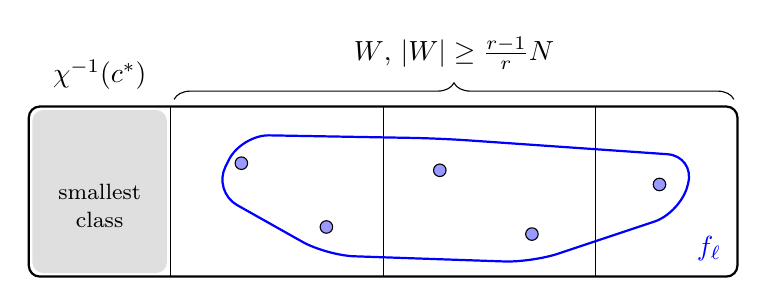
\begin{tikzpicture}[vtx/.style={circle,draw,inner sep=1.6pt}, scale=0.9]
	\draw[thick,rounded corners] (0,0) rectangle (10,2.4);
	\draw (2,0) -- (2,2.4); \draw (5,0) -- (5,2.4); \draw (8,0) -- (8,2.4);
	\fill[gray!25,rounded corners] (0.05,0.05) rectangle (1.95,2.35);
	\node at (1,2.85) {$\chi^{-1}(c^*)$};
	\draw[decorate,decoration={brace,amplitude=6pt}] (2.05,2.5) -- (9.95,2.5);
	\node at (6,3.15) {$W$, $|W| \ge \frac{r-1}{r} N$};
	\node[font=\footnotesize] at (1,1.2) {smallest};
	\node[font=\footnotesize] at (1,0.8) {class};
	\foreach \x/\y in {3/1.6, 4.2/0.7, 5.8/1.5, 7.1/0.6, 8.9/1.3} \node[vtx,fill=blue!40] at (\x,\y) {};
	\draw[blue,thick,rounded corners=10pt] (2.6,1.2) -- (3,2) -- (5.8,1.95) -- (9.4,1.7) -- (9.2,0.9) -- (7.1,0.2) -- (4.2,0.3) -- cycle;
	\node[blue] at (9.6,0.4) {$f_\ell$};
\end{tikzpicture}
\caption{For a fixed colouring $\chi$, any edge $f_\ell \subseteq W$ misses the colour $c^*$ and so is not rainbow.}
\label{fig:ex5}
\end{figure}

% \newpage

% \section*{Hints}  The following QR codes contain hints for some of the homework exercises.  You should be able to decode them using any QR code scanner, including this one: \url{https://zxing.org/w/decode.jspx}.

% \paragraph{Exercise ?} Also available at \url{https://i.ibb.co/???????/S??E?.png}.

\begin{center}
% \includegraphics[scale=0.5]{Hints/S??E?.png}
\end{center}

\end{document}